\documentclass{article}
\usepackage{graphicx}
\begin{document}

\begin{center}
\section*{\LARGE Calculus For Dummies}
\subsubsection*{By Mark Ryan}
\newpage
\section*{Introduction}

\end{center}
Much of calculus is really just very
advanced algebra, geometry, and trig. It builds upon and is a logical extension of those subjects. If you can do \textbf{algebra}, \textbf{geometry}, and \textbf{trig}, you can do
\textit{calculus}.

\begin{center}
    \part{An Overview of Calculus}
    \begin{itemize}
        \item A brief and straightforward explanation of just what calculus is.
        Hint: it’s got a lot to do with \textbf{curves} and with things that are
        \textbf{constantly changing}.

        \item Examples of where you might see calculus at work in the real
        world: curving cables, curving domes, and the curving path of a
        spacecraft.
        \item The first of the two big ideas in calculus: \textbf{differentiation}, which
        means finding a \textbf{derivative}. A derivative is basically just the
        fancy calculus version of a \textbf{slope}; and it’s a simple rate — a this
        per that.
        \item The second big calculus idea: \textbf{integration}. It’s the fancy calculus
        version of adding up small parts of something to get the total.
        \item An honest-to-goodness explanation of why calculus works: In
        short, it’s because when you \textbf{zoom in on curves} (infinitely far),
        they become \textbf{straight}.
    
    \end{itemize}

  
\end{center}
\newpage

\section{\LARGE What Is Calculus?}
\vspace*{5mm}
Calculus is basically just advanced algebra and geometry. It can be seen as an extension of these two fields of study.\\
\\
For instance, in figure 1, the man in the left image is pushing a box up a straight incline.
On the right however, the man is pushing up the same box up a curving incline. The problem in both cases is to determine the amount of energy required to push the crate up the slope.

\begin{figure}[h]
    \centering
    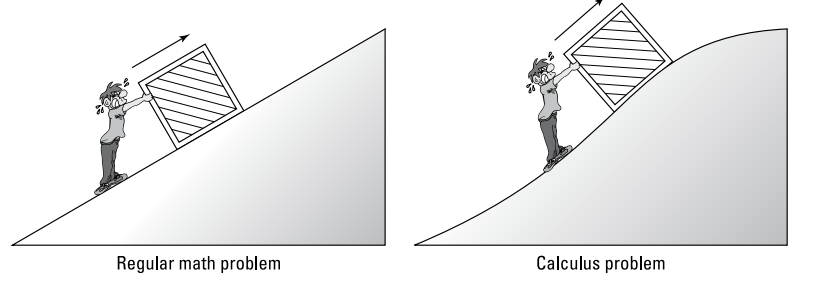
\includegraphics[width=1.1\textwidth]{figure-1-1.png}
    \caption{The difference between regular math and calculus: In a word, it’s the curve}
    \label{fig:01}
\end{figure}

\subsubsection*{\large Work Done}
\begin{center}
$W = F * d$

\end{center}
``Work done'' is concerned with the energy transferred from one object to another as a result of a force applied over a distance. So let's say we apply a force of 20N to a box over a distance of 0.5m, the amount of work done would be equal to 10 Joules.
This is all nice and dandy, but what if we want to calculate the amount of work done when the force applied is \textbf{not constant} - this is where calculus comes into play. 

\subsubsection*{\large Straight Incline}
For the straight line, the man is pushing the box with an \textit{unchanging force}, and the crate goes up the incline at an \textit{unchanging speed}. With some si,ple physics formulas and regular math (includig algebra and trigonometry), you can compute how many caloriesof energy are required to push the crate up the incline slope.\\
\textbf{*The amount of energy expended each second remains the same}


\subsubsection*{\large Curving Incline}
For the curving incline, things are \textit{constantly} changing. The steepness of the incline is \textit{changing} - and not just in increments (one steepness for the first 3 feet then a different steepness for the next 3 feet).
It's \textit{constantly changing}. The man is also pushing the box in \textit{constantly changing force} - the steeper the incline the harder the push.
As a result, the amount of energy expended is also changing, not every second or every thousandth of a second, but constantly changing from one moment to the next. That’s
what makes it a calculus problem. By this time, it should come as no surprise to you that calculus is described as “\textit{the mathematics of change}.” 
\\
\\
For the curving incline problem, the physics formulas remain the same, and the
algebra and trig you use stay the same. The difference is that — in contrast to
the straight incline problem, which you can sort of do in a single shot — you’ve
got to break up the curving incline problem into small chunks and do each chunk
separately. Figure 1-2 shows a small portion of the curving incline blown up to
several times its size.

\begin{figure}[h]
    \centering
    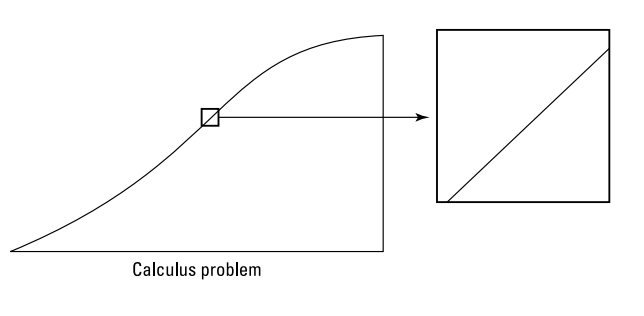
\includegraphics[width=0.8\textwidth]{figure-1-2.png}
    \caption{Zooming in on the curve — voilà, it’s straight (almost).}
    \label{fig:02}
\end{figure}

What makes the invention of calculus such a fantastic achievement is that it
does what seems impossible: it zooms in infinitely. As a matter of fact, everything in calculus involves infinity in one way or another, because if something
is constantly changing, it’s changing infinitely often from each infinitesimal
moment to the next.

\newpage
\subsection*{\LARGE Real-World Examples of Calculus}
With regular math we can determine the length of a straight line that runs diagonally from one point to another using Pythagorean theorem.
With calculus we can determine the length of of a curved line.See Figure 3.
\begin{figure}[h]
    \centering
    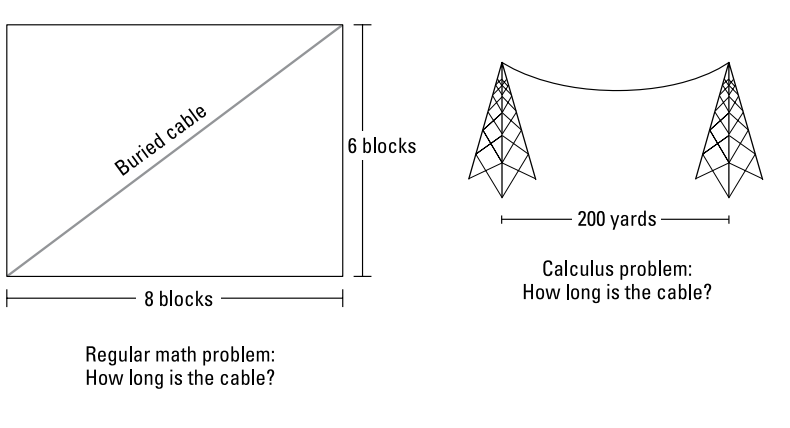
\includegraphics[width=1\textwidth]{figure-1-3.png}
    \caption{Without and with calculus.}
    \label{fig:03}
\end{figure}

We can also calculate the area of domes and other circular structures. See Figure 4.
\begin{figure}[h]
    \centering
    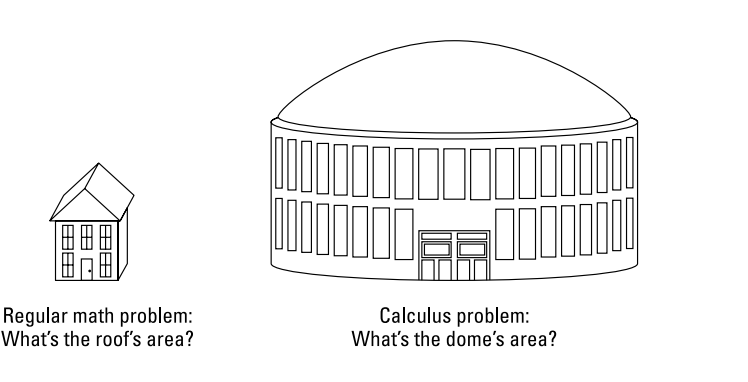
\includegraphics[width=0.8\textwidth]{figure-1-4.png}
    \caption{Without and with calculus.}
    \label{fig:03}
\end{figure}

\newpage


\section{\LARGE The Two Big Ideas of Calculus: \\Differentiation and Integration — \\plus Infinite Series}
\vspace*{5mm}
\end{document}